\documentclass{beamer}
\usepackage[T1]{fontenc}
\usepackage[utf8]{inputenc}
\usepackage{lmodern}
\usepackage[polish]{babel}
\usepackage{graphicx}
\usepackage{multirow}

\usetheme{AGH}

\title[Interpolacja barwna obrazu]{Równoległa interpolacja obrazu barwnego
  z~kamery cyfrowej}

\author[B. Bułat, T. Drzewiecki]{Bartłomiej Bułat, Tomasz Drzewiecki}

\date[2011]{24.01.2012}

\institute[AGH]
{Wydział EAIiIB\\ 
Katedra Automatyki i~Inżynierii Biomedycznej
}

\setbeamertemplate{itemize item}{$\maltese$}

\begin{document}

{
\usebackgroundtemplate{
\includegraphics[width=\paperwidth]{titlepagepl}} % wersja polska
 \begin{frame}
   \titlepage
 \end{frame}
}

%---------------------------------------------------------------------------

%% Figure example
%\begin{figure}
%  \includegraphics[width=0.5\textwidth]{filename}
%  \caption{Figure caption}
%  \label{fig:label}
%\end{figure}

\begin{frame}
\frametitle{Plan prezentacji}
	
  \begin{itemize}
  	\item Cele projektu
	  \item Wstęp teoretyczny
  	\item Programowanie w~OpenCL
  	\item Framework
	\item Testowanie
  	\item Podsumowanie
	\end{itemize}

\end{frame}

\begin{frame}
	\frametitle{Cele projektu}
	
  Celem projektu była implementacja algorytmu interpolacji barwnej obrazu z~kamery
  z~użyciem zrównoleglania obliczeń na~karcie graficznej (OpenCL). 
  
  Wynikiem prac miała być
  biblioteka realizująca wymieniony algorytm, biblioteka obsługująca kamerę wysokiej rozdzielczości
  oraz aplikacja integrująca obie biblioteki pozwalająca na~przetwarzanie obrazu z~kamery w~czasie 
  rzeczywistym.  
\end{frame}

\begin{frame}
  \frametitle{Matryca Bayer-a}
  
  \begin{columns}
  \begin{column}{5cm}
  Kamery używają pewnej topologii filtrów kolorowych na~matrycy. Matryca Bayer-a to topologia odzwierciedlająca
  sposób postrzegania kolorów przez ludzkie oko. Na rysunku obok pokazano powiększony układ
  filtrów na~tej matrycy.
  \end{column}
  \begin{column}{5cm}
    \begin{center}
    \begin{figure}

	  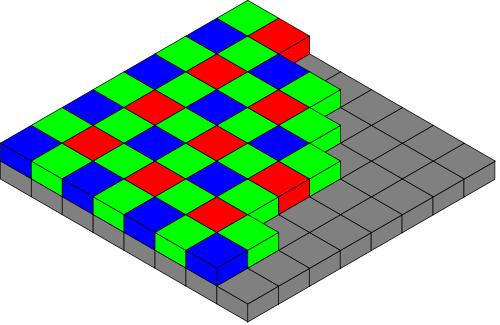
\includegraphics[width=\textwidth]{bayer_pattern_sensor}
	  \caption{Układ filtrów kolorowych na~matrycy Bayer-a}
	  \label{fig:pattern}
    \end{figure}
    \end{center}
	\end{column}
	\end{columns}
	
\end{frame}

\begin{frame}
	\frametitle{Interpolacja barwna}
	
	\begin{columns}
	\begin{column}{4cm}
    \begin{center}
    \begin{figure}

	  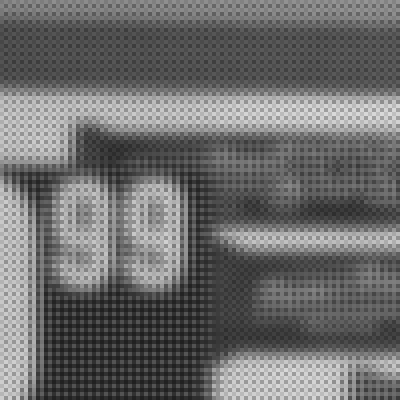
\includegraphics[width=\textwidth]{raw_image}
	  \caption{Surowy obraz z~matrycy Bayer-a}
	  \label{fig:raw_image}
    \end{figure}
    \end{center}
  \end{column}
  \begin{column}{6cm}
	Na rysunku obok przedstawiony jest powiększony fragment obrazu surowego, odczytanego prosto z~matrycy.
	Aby przekształcić taki obraz w~obraz kolorowy, należy dla każdego piksela interpolować wartość kolorów:
	{\color{red}czerwonego}, {\color{green}zielonego} oraz {\color{blue}niebieskiego}.
	
	Interpolacja wykonywana jest z~wykorzystaniem wartości pikseli sąsiednich.
  \end{column}
  \end{columns}
\end{frame}

\begin{frame}
	\frametitle{Kontekst sąsiedztwa}
	
	W algorytmie interpolacji wykorzystaliśmy 3 konteksty sąsiedztwa, znajdujące się na~obrazku poniżej. Im mniejsze sąsiedztwo tym szybsze obliczenia, lecz bardziej poszarpane krawędzie na~obrazie. Im większe sąsiedztwo, tym bardziej wygładzony obraz lecz wolniejsze obliczenia.
	
  \begin{figure}
  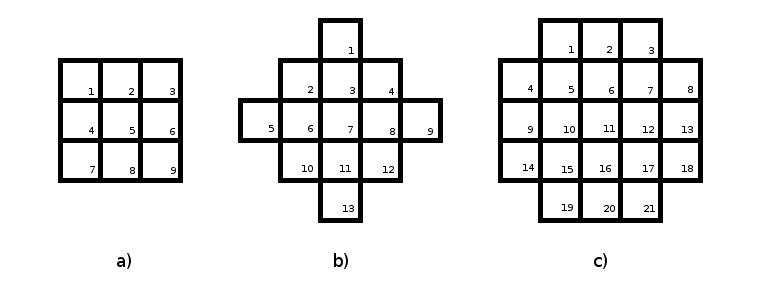
\includegraphics[width=0.5\textwidth]{masks}
  \caption{Wykorzystane konteksty sąsiedztwa. a) sąsiedztwo 3x3, b)~sąsiedztwo~,,koło'',
  c)~sąsiedztwo ,,krzyż''}
  \label{fig:masks}
  \end{figure}
\end{frame}

\begin{frame}
  \frametitle{Algorytm interpolacji}
  \emph{Na przykładzie maski 3x3:}
  
  \begin{enumerate}
    \item Określenie konfiguracji kolorów na~podstawie aktualnego przesunięcia piksela i~określonej
      początkowej konfiguracji matrycy,
    \item Wyliczenie średniej wartości dla każdego koloru należącego do~kontekstu,
    \item Przypisanie obliczonych wartości średnich do~odpowiednich kolorów.
  \end{enumerate}
  
  \begin{figure}
  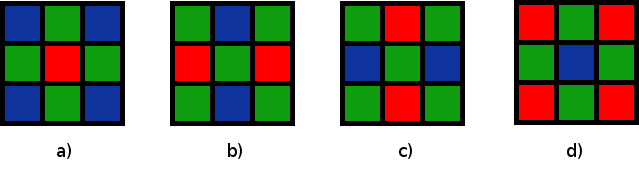
\includegraphics[width=0.5\textwidth]{mask3conf}
  \caption{Możliwe konfiguracje pikseli w~kontekście sąsiedztwa 3x3.}
  \label{fig:masks}
  \end{figure}
  
\end{frame}

\begin{frame}
	\frametitle{Programowanie w~OpenCL}
	
	\emph{\textbf{OpenCL} - otwarty standard dla wieloplatformowego, równoległego programowania współczesnych procesorów w~komputerach osobistych\footnote{Za stroną www.khronos.org/opencl/}.}
	
	\vspace{1em}
	
	Założenia programowania w~OpenCL:
	
	\begin{itemize}
	\item Programowanie \emph{kerneli}, wykonywanych dla każdego elementu obrazu (tablicy danych),
	\item Wykonanie następuje możliwe równolegle (zależnie od dostępnej architektury),
	\item Używana jest dzielona pamięć danych.
  \end{itemize}
\end{frame}

\begin{frame}
  \frametitle{Implementacja kontrolera po stronie CPU}
  W~celu łatwiejszej, szybszej oraz generującej mniej błędów implementacji stworzono mały framework klas realizujących obsługę OpenCL od strony procesora.
Schemat jego struktury jest przedstawiony na~rys. \ref{fig:class_diagram} na~następnym slajdzie.
\end{frame}

\begin{frame}
  \frametitle{Diagram klas}
\begin{figure}
  \centering
  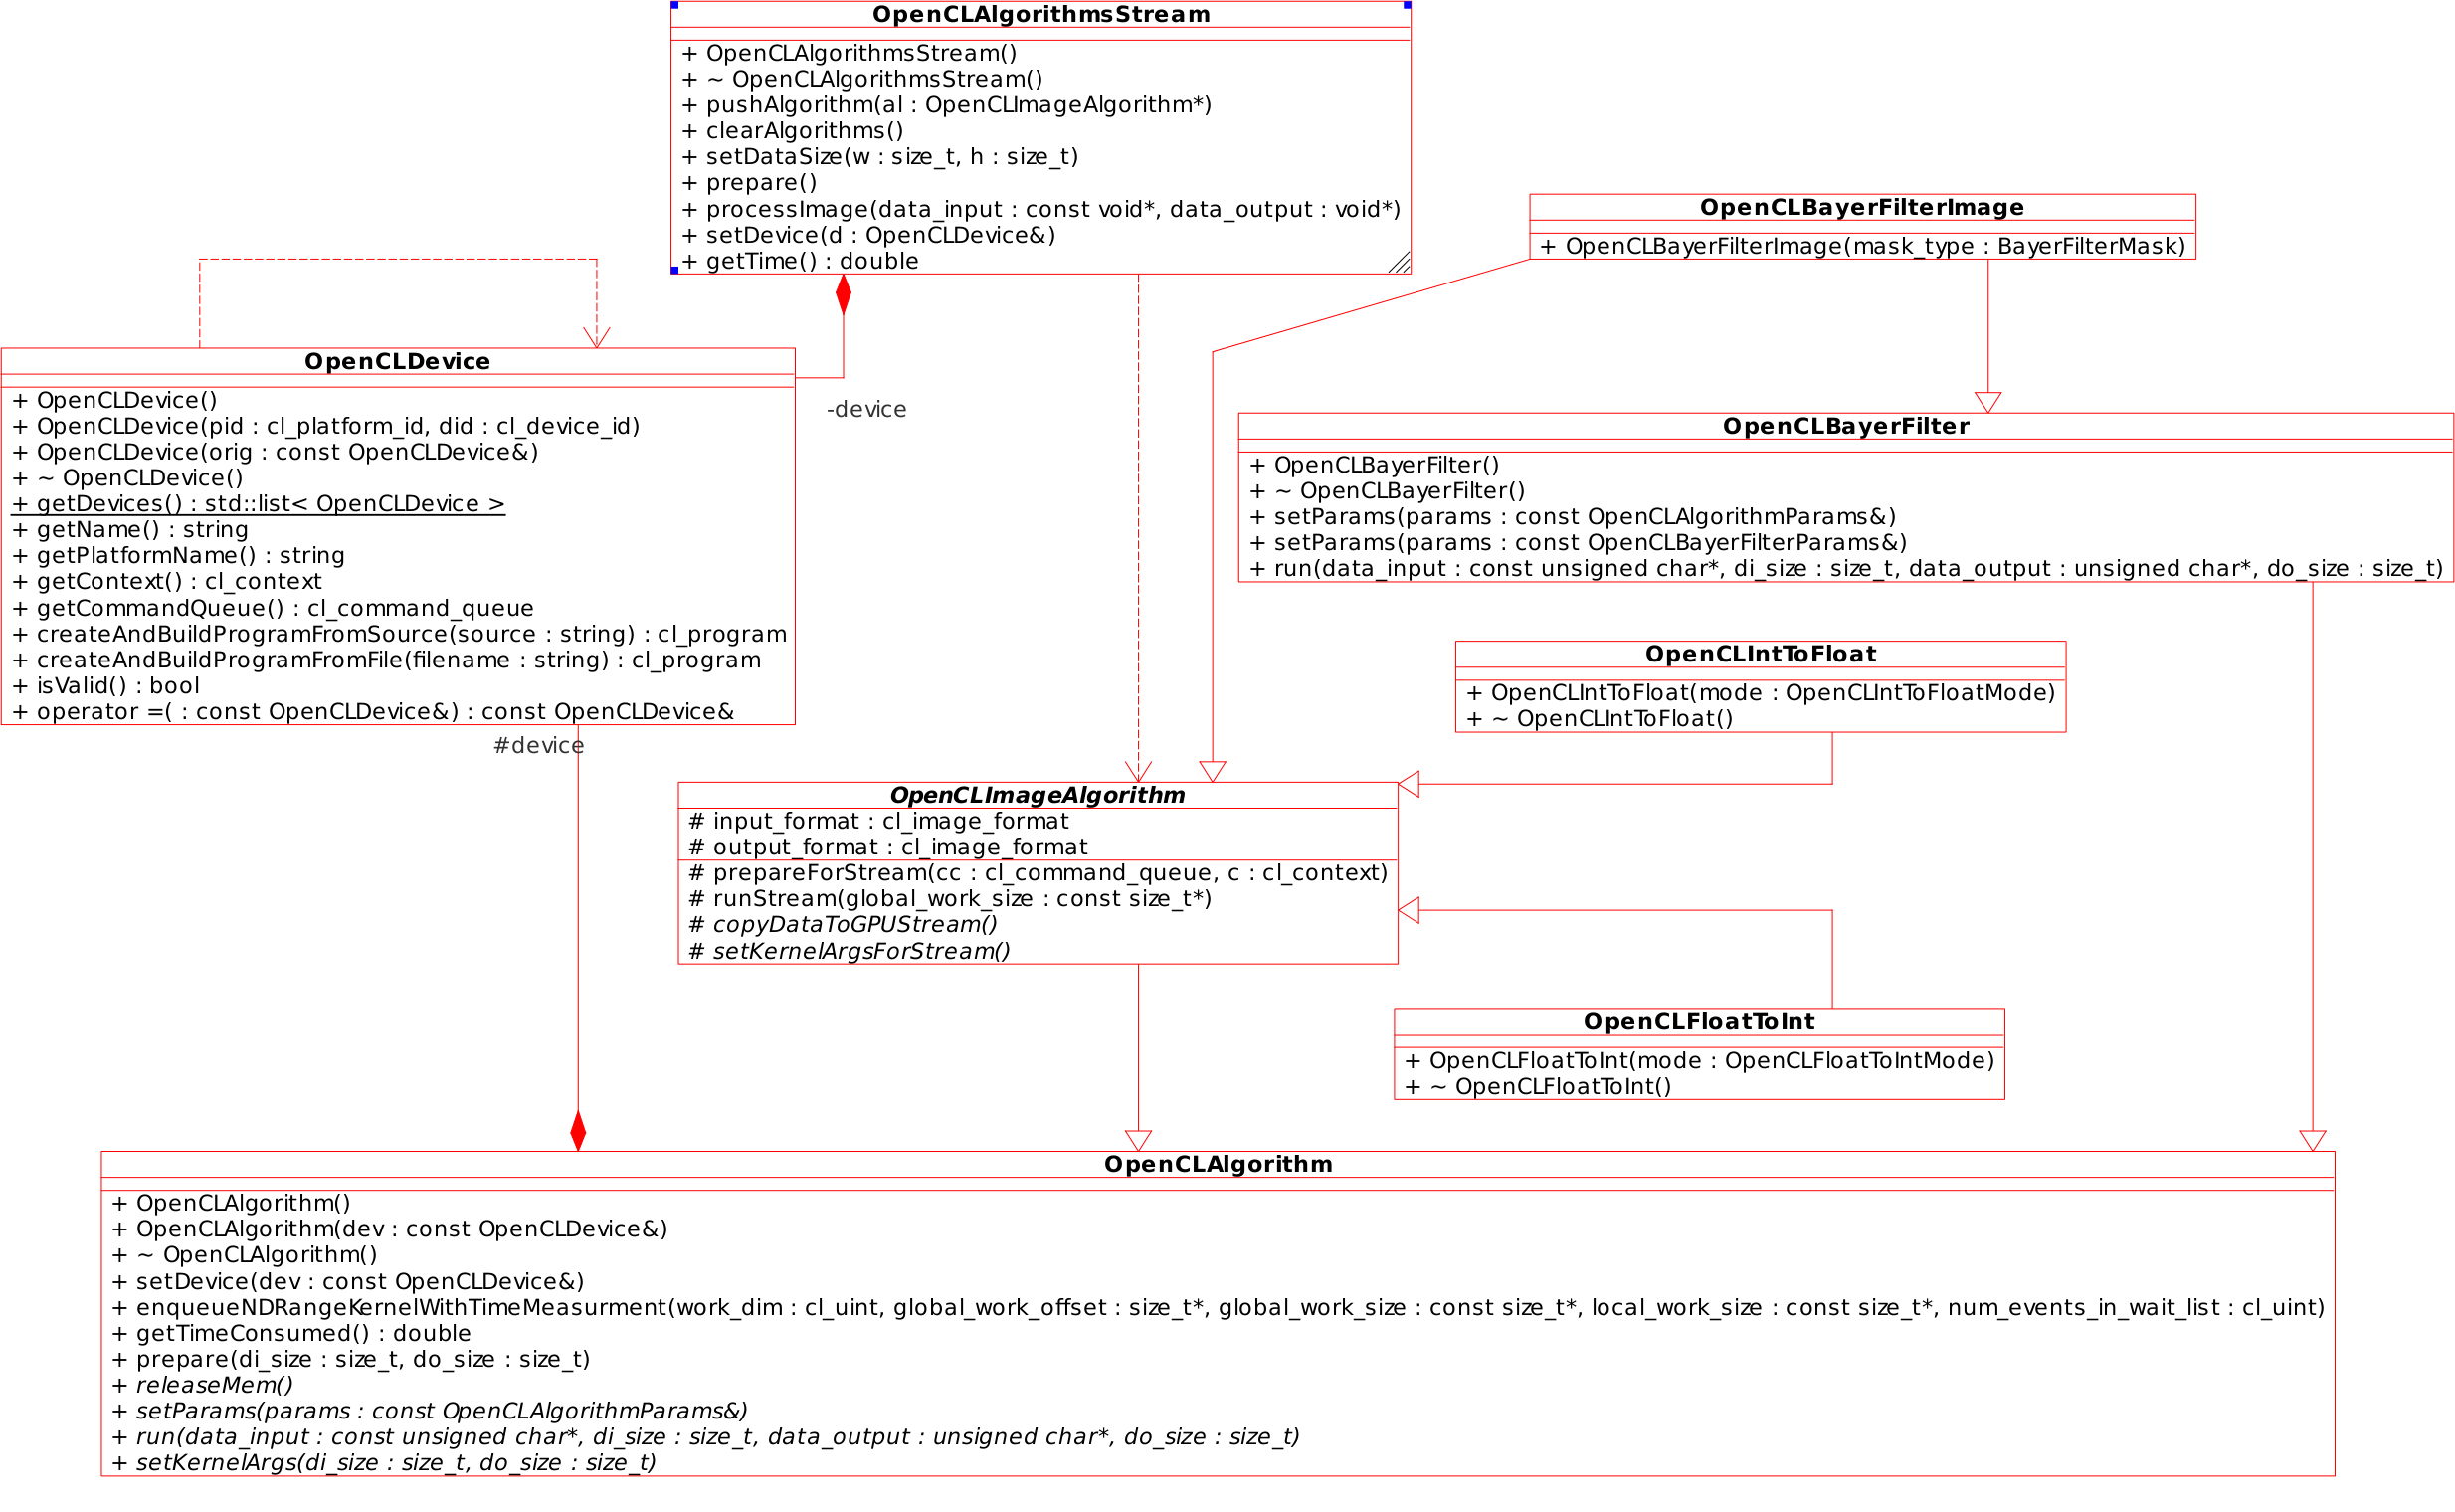
\includegraphics[width=0.9\linewidth]{class_diagram}
  \caption{Diagram klas stworzonego frameworku.}
  \label{fig:class_diagram}
\end{figure}
  
\end{frame}

\begin{frame}
  \frametitle{Testowanie poprawności działania algorytmu}

W celu określenia poprawności algorytmu porównano obraz wynikowy z~istniejącą implementacją zrealizowaną na~procesorze. Do sprawdzenia wybrano implementację zrealizowaną w~OpenCV. Wyniki porównań przedstawiono na~rysunku na~następnym slajdzie.

\end{frame}

\begin{frame}
  \frametitle{Testowanie poprawności działania algorytmu}
\begin{figure}
  \centering
  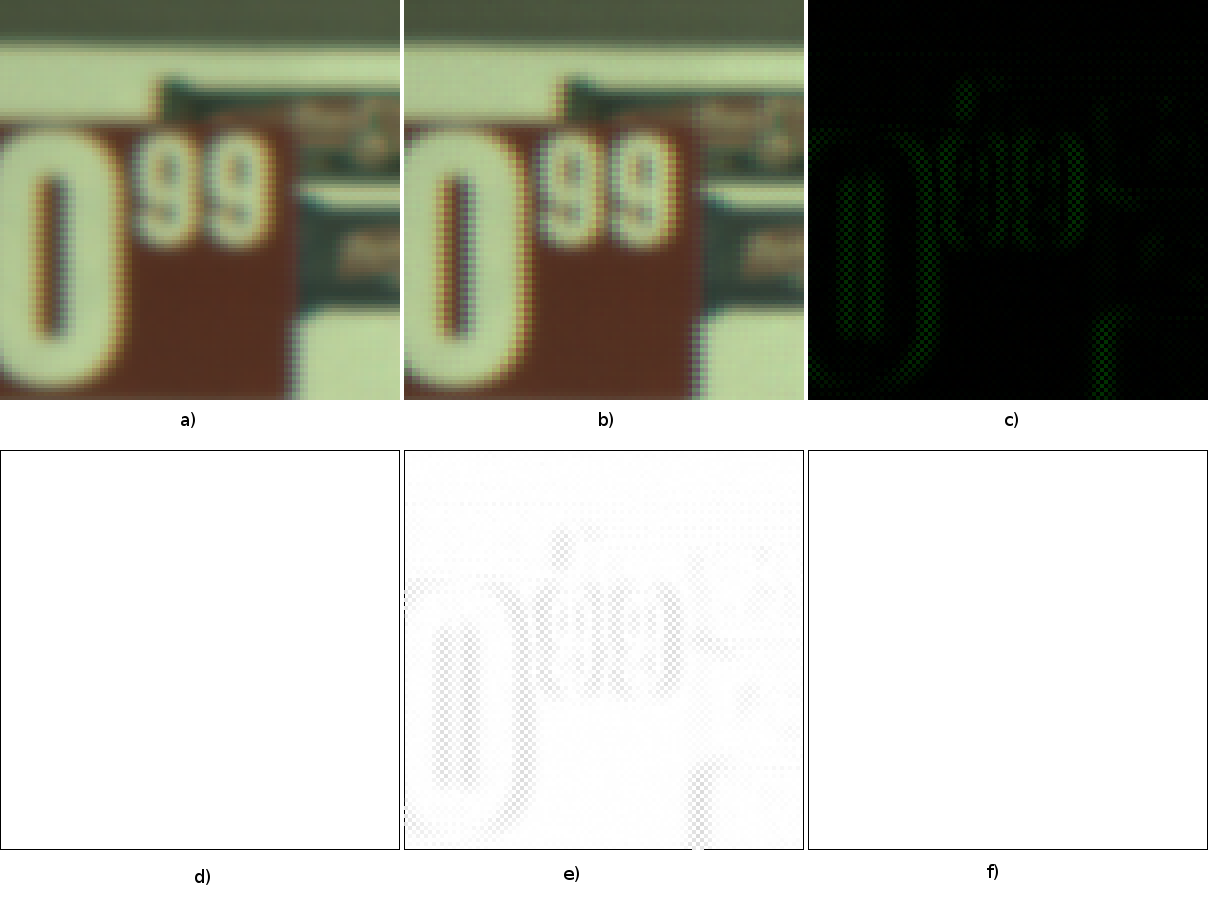
\includegraphics[width=0.55\linewidth]{result_diff}
  \caption{Fragment wynikowego obrazu z~implementacji w~OpenCL (a), implementacji w~OpenCV (b) oraz różnicy obrazów (c). Obraz (d) przedstawia różnice koloru czerwonego, (e) zielonego, a~(f) niebieskiego.}
  \label{fig:result_diff}
\end{figure}
\end{frame}

\begin{frame}
  \frametitle{Testowanie - sprzęt}
  Testy szybkości algorytmu zostały zrealizowane z~użyciem dwóch kart graficznych o~parametrach:
\begin{center}
\begin{table}
  \caption{Porównanie kart graficznych użytych do~testów.}
  \label{tab:gpus}
     \begin{tabular}{ |l | r | r | }
     \hline
       & GT 555M & GT9800 \\ \hline
     Liczba rdzeni & 144 & 128 \\ \hline
     Częstotliwość rdzenia & 1250MHz & 600MHz \\ \hline
     Częstotliwość pamięci & 1800MHz & 900MHz \\ \hline
     Magistrala pamięci & 128bit & 256bit \\ \hline

   \end{tabular}

\end{table}
\end{center}
Do obliczeń referencyjnych użyto procesora Intel Core i7-2670QM 2,2GHz.
\end{frame}

\begin{frame}
  \frametitle{Testowanie - procedura}
\begin{itemize}
  \item Algorytmy testowano na~79 obrazach o~wymiarach 2546x2058 pikseli.
  \item Do każdego testu użyto tych samych obrazów, które były zapisane na~dysku. Czas odczytywania obrazów z~plików nie był doliczany do~czasu obliczeń.
  \item Liczono czas wykonania wszystkich operacji koniecznych do~wykonania algorytmu (np. kopiowanie do~pamięci karty graficznej) oraz osobno czas wykonania kerneli.
  \item Jako czas referencyjny został użyty czas wykonania obliczeń implementacji algorytmu w~bibliotece OpenCV wykonanej na~procesorze.

\end{itemize}


\end{frame}


\begin{frame}
  \frametitle{Testowanie - wyniki}
\begin{center}
\begin{table}
  \caption{Wyniki testów. A) czas obliczeń, B) czas na~jeden obraz, C) czas wykonania kerneli oraz
    D) czas wykonania kerneli na~jeden obraz.}
  \label{tab:test_Result}
   \begin{tabular}{ | c | c | c | c | c | c | c | c | }
     \hline
 & OpenCV & \multicolumn{3}{ |c|}{GeForce 555M} & \multicolumn{3}{ |c|}{GeForce 9800GT} \\ \cline{3-8}
       &  & a) & b) & c) & a) & b) & c)  \\ \hline
A    		& 2,548s & 2,139s & 3,107&2,309 &4,914 & 6,162&8,947 \\ \hline
B    	& 0,032s &
0,027s &
0,039s &
0,029s &
0,062s &
0,078s &
0,113s \\ \hline
C    	& & 
1,467s &
2,462s &
1,571s &
4,301s &
4,499s &
7,837s
 \\ \hline
D    & & 
0,018s &
0,031s &
0,020s &
0,054s &
0,057s &
0,099s
\\ \hline
   \end{tabular}
\end{table}
\end{center}
\end{frame}


\begin{frame}
  \frametitle{Analiza wyników}
\begin{itemize}
	\item Można zauważyć, że jest duża różnica w~czasie obliczeń pomiędzy kartami graficznymi. Jest to spowodowane parametrami kart.
	\item Dodatkowo trzeba wziąć pod uwagę, że karta 555M jest kartą wyprodukowaną znacznie później niż karta 9800GT. Karty są ciągle ulepszane, technologie się rozwijają, więc nawet jeśli nie widać znaczących zmian w~parametrach danej karty.

	\item Porównując implementację referencyjną, używającą maski a) można zaobserwować przyśpieszenie przetwarzania. Również obliczenia dla maski c) zajęły mniej czasu.
\end{itemize}
\end{frame}

\begin{frame}
  \frametitle{Podsumowanie}
  Udało się zrealizować wyznaczone cele. Implementacja algorytmu interpolacji barwnej została zrealizowana z~użyciem OpenCL. W~porównaniu do~innych, już sprawdzonych, implementacji osiągnięte wyniki są zadowalające w~aspekcie poprawności oraz czasu obliczeń.
\end{frame}

\begin{frame}
  \frametitle{Koniec}
\begin{center}
Dziękujemy za uwagę.
\end{center}
\end{frame}

\end{document}

